\section{Implementation} \label{sec:implementation}
\yueqiang {
implementations:
1) hooks for on-demand enable
2) locks for mechanism
3) data structures in mechanism
4) threshold selection for cache free? or this discussed in design
5) }

Based on Xen version 4.2.1 and guest kernel version 3.2.0-rc1, \name implements the access control related to cache flag as well as management of page-table cache.

\subsection{Cache Flag}

From a 32-bit field related to page type information, \name was planning to use a redundant bit to represent the cache flag in order to be compatible with its original implementation. However, each bit in the upper 9-bit of the field has its specific use and the lower 23-bit serves as the reference count of current page type, representing at most ($2^{23}-1$) reference counts of the page type (see figure ~\ref{fig:subfig:a}). \name enforces a stricter rule to prevent count overflow, as cache flag occupies the top bit of the 23-bit and the maximal reference count is limited to ($2^{22}-1$), which affects Xen little (see figure ~\ref{fig:subfig:b}). Actually, Xen hypervisor is functioning well with the flag bit since the reference count of a page type during runtime cannot reach at ($2^{22}-1$). On top of that, \_\_get\_page\_type() is the critical function to be customized in order to check if a machine page has the flag bit.

\begin{figure}
\centering
\subfigure[Existing Representation]{
\label{fig:subfig:a}
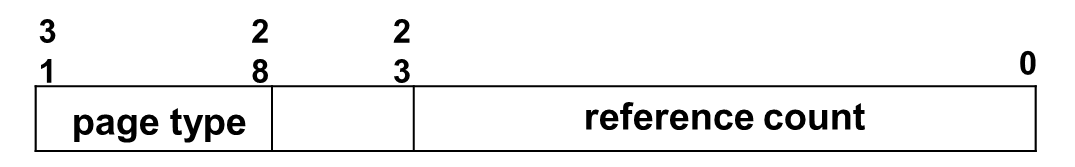
\includegraphics[width=0.5\textwidth]{image/implementation/field-of-page-type-info.png}}
\hspace{1in}
\subfigure[Cache Flag Representation]{
\label{fig:subfig:b}
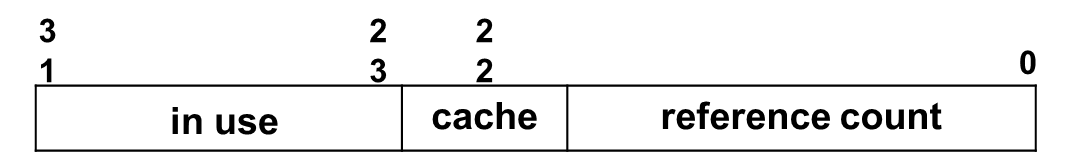
\includegraphics[width=0.5\textwidth]{image/implementation/field-of-page-type-info-with-cache-flag.png}}
\caption{Field of Page Type Info}
\label{fig:PGtime} %% label for entire figure
\end{figure}

\subsection{Management of Page Table Cache}

In the PV setting, guest OS is required to work in PAE (i.e., Physical Address Extension) mode. As a result, \name maintains three levels of cache pools, each of which is essentially a structured single-linked list caching the guest physical addresses of pages. For the top two levels used for caching PGD (i.e., Page Global Directory) and PMD (i.e., Page Middle Directory), \name obtains the physical addresses directly from their linear addresses. While the bottom PT (i.e., Page Table) is located in the High Memory, the mapping between its linear and physical addresses is not stable. \name acquires the physical addresses of cached PT pages from the corresponding page-info structures.

Every list supports operations of both removal and insertion. Removal exists within the cache allocating function, which fetches a cached page from the top of the list. Insertion is located within the cache freeing function, which inserts a cached page also onto the top. Also, \name maintains two global operation counters, namely num\_in\_use and num\_in\_pool, each logging the invocation times of removal and insertion, respectively. They are required when cache freeing function needs to free cached pages into the buddy system. Every pair of cache allocating and freeing functions is used to hook existing page-table related functions. By this way, whenever OS creates or destroys any process, it always interacts with the caches. Also note that every cache pool and operation counter are shared data resources and their related operation code are critical sections. \name makes use of locks to ensure exclusive resource-access in the multi-processor setting. More specifically, Every level of page-table cache and all its operation counters share a spin lock and irrelevant operations should be removed out of the critical section, especially those that are time-consuming.

\name implements a new system call to provide an interface for users to activate the cache in an on-demand way. In the system call, a global boolean variant is defined, which is initialized as false, indicating that cache is not enabled. And users can assign the variant as true to enable the cache. Anther two user interfaces related to modification of default thresholds and freeing all pages in cache are also implemented through system calls. For the modification, new thresholds of the proportion and total page number are passed as agruments while users can frees all cached pages by resetting a global boolean variant, which is initialized as true.

Within the cache freeing function, a hypercall is implemented with a single-linked list of cached addresses of pages as the parameter. The hypercall is a uniform interface for every level of cache freeing function, simplifying the modifications both to guest OS and Xen. As a reply to the hypercall, Xen mainly zeroes the flag bit of 32-bit field and invokes the important function interface intel\_iommu\_map\_page to create entries in the I/O page tables as well as flush IOTLB.




